\documentclass[a4paper,12pt]{book}

\usepackage[utf8]{inputenc}
\usepackage[brazil]{babel}
\usepackage{geometry}
\usepackage{setspace}
\usepackage{indentfirst}
\usepackage{hyperref}
\usepackage{graphicx}
\usepackage{listings}
\usepackage{xcolor}
\usepackage{enumitem}
\usepackage{tikz}
\usepackage{verbatim}
\usepackage{caption}
\usepackage{subcaption}


\setlist[itemize]{itemsep=0pt}

% Configurações da página
\geometry{
	a4paper,
	top=2.5cm,
	bottom=2.5cm,
	left=3cm,
	right=2.5cm
}

% Espaçamento entre linhas
\onehalfspacing

% Recuo da primeira linha dos parágrafos
\setlength{\parindent}{1.25cm}

\hypersetup{
	colorlinks=true,
	linkcolor=blue,
	filecolor=blue,
	urlcolor=blue,
	citecolor=blue,
	anchorcolor=blue,
	breaklinks=true,
	pdftitle={Aprendizagem de máquina básico: uma abordagem teórico-prática com Python},
	pdfauthor={Giseldo Neo},
	pdfsubject={Aprendizagem de máquina básico: uma abordagem teórico-prática com Python},
	pdfkeywords={aprendizagem de máquina},
	pdfcreator={LaTeX},
	pdfproducer={pdfTeX},
	pdfstartview={FitH},
	pdfpagemode={UseOutlines},
	pdfpagelayout={SinglePage}
}

\lstset{
	basicstyle=\ttfamily\footnotesize,
	keywordstyle=\color{blue},
	commentstyle=\color{green},
	stringstyle=\color{red},
	numbers=left,
	numberstyle=\tiny\color{gray},
	stepnumber=1,
	numbersep=10pt,
	backgroundcolor=\color{white},
	showspaces=false,
	showstringspaces=false,
	showtabs=false,
	frame=single,
	tabsize=2,
	captionpos=b,
	breaklines=true,
	breakatwhitespace=false,
	escapeinside={\%*}{*)}
}

\author{Giseldo Neo}
\title{Aprendizagem de máquina básico: uma abordagem teórico-prática com Python}

\begin{document}

	\newcommand{\titlepagecolor}{cyan!20}

	\begin{titlepage}
		\begin{tikzpicture}[remember picture,overlay]
			\fill[\titlepagecolor] (current page.south west) rectangle (current page.north east);
		\end{tikzpicture}

		\begin{center}
			{\Huge\bfseries Aprendizagem de máquina básico: uma abordagem teórico-prática com Python}\\[1.5cm]

			
\includegraphics[width=1\textwidth]{figuras/capa2.jpg}\\[1cm]

			{\Large Giseldo Neo}\\
			{\small versao alpha 0.1}\\
			{\small\today}\\
			{\small \textsuperscript{\textcopyright} Todos os direitos reservados}\\
		\end{center}
	\end{titlepage}

\tableofcontents

\chapter{Introdução}

\section{Inteligência artificial}

O termo ``inteligência'' tem várias definições que dependem do contexto. Isso pode trazer certa confusão no entendimento e delimitação do tema. Menos abrangente, porém mais confuso ainda, é o termo ``inteligência artificial''. Portanto, dado as diversas definições de inteligência artificial (IA), ou \textit{artificial inteligence} em inglês vamos delimitar um pouco o significado das palavras.

Nós humanos somos da espécie Homo-Sapiens. Espero que o leitor ainda o seja, pois esse texto pode estar sendo processado para treinar o mais novo modelo de IA, como por exemplo, o Gemini da Google, o chatGPT da openAI ou o copilot da Microsoft.

%como a do filme ``2001 uma odisseia no espaço'', clássico de Kubric, ou como a do mais recente filme ``Ela'', com o ator Joaquim Phenix, espero que com sorte, por um garoto interessado em aprender.

Homo-Sapiens vem do latim e significa homem sábio \cite{wikipediahumano}. A importância da sapiência (que é um sinônimo de inteligência) é tamanha que define a nossa própria espécie. Porém, neste contexto consideramos que um gato e um cachorro são seres dotados de inteligência, uma abelha, então nem se fala, praticamente uma cientista. Portanto, seremos mais contidos e reservados quanto ao termo inteligência.

Além disso, várias questões relacionadas a inteligência também guiam inúmeras outras pesquisas cientificas e filosóficas, por exemplo: como funciona nossa inteligência? Nossa percepção do ambiente é próxima da realidade objetiva? Porém, ainda não é dessa inteligência que estamos falando. Essas perguntas estão mais próxima da neurociência e da filosofia.

O que confunde bastante é que ``inteligência'' e ``artificial'' são palavras que têm significado implícito para pessoas que não são da área de computação, naturalmente surge o desejo de médicos, advogados, engenheiros (só para citar alguns) de verificar como a “inteligência artificial” pode ser inserida na sua rotina diária. Por exemplo, o meu dentista já quis saber como a IA iria afetar seus procedimentos odontológicos. Porém, ninguém nunca me perguntou em como a ``Transformada de Fourier'' poderia melhorar o seu dia-a-dia, mesmo sabendo que ela já é utilizada em vários domínios do conhecimento e com entusiasmo \cite{wikipediafourier}.

A ``inteligência artificial'' mais próxima da computação está mais relacionada com a capacidade de realizar coisas que seres inteligentes (um gato, um bebê, ou um cientista) realizam, como por exemplo puxar a mão (ou pata) instantaneamente ao tocar em uma superfície quente (inteligência reativa), ou realizar uma prova de anatomia (inteligência cognitiva). Se conseguimos que programas realizem ações realizadas por entidades dotadas de inteligencia, e realizamos isso  de forma computacional, estamos próximos do significado desejado de ``inteligência artificial''.

Russel e Norvig (2020) em um dos livros mais lidos em todas as universidades do mundo tem uma boa definição: ``O campo da inteligência artificial [...] tenta não apenas compreender, mas também construir entidades inteligentes'' (tradução nossa) \cite{norvig2002}.  Em outras palavras temos o audacioso objetivo de construir agentes dotados dessa inteligência.

A origem do termo ``inteligência artificial'', neste contexto, é atribuída a John McCarthy, professor de Matemática da Universidade Dartmouth College \cite{blipblog}, ele organizou uma conferência com duração de oito semanas com mais alguns colegas em 1956, alguns anos após a segunda guerra, e desde então o termo vem sendo utilizado para designar parte de conteúdos estudados em ciência da computação. Porém, um pouco antes, o artigo seminal de Alan Turing já demonstrava um bom ensaio sobre as possibilidades de uma máquina possuir inteligência \cite{Turing1950}.


\begin{figure}[h]
    \centering
    \begin{subfigure}[b]{0.45\textwidth}
        \centering
        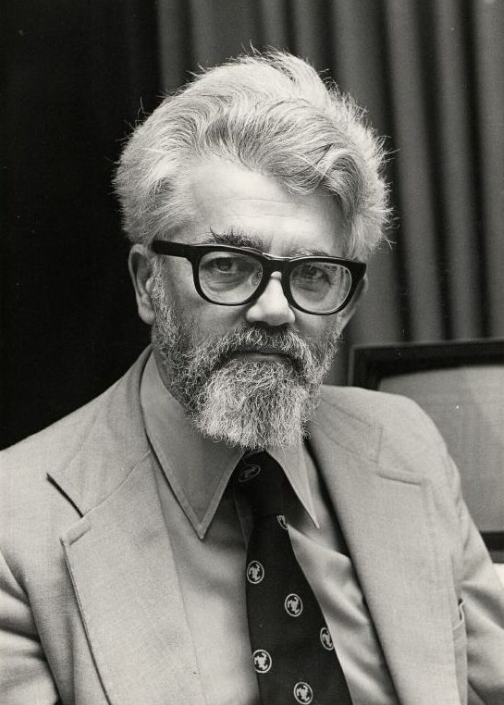
\includegraphics[width=0.5\linewidth]{figuras/jhon_macharthy}
		\caption{Jhon MacCarthy}
        \label{fig:image1}
    \end{subfigure}
    \hfill
    \begin{subfigure}[b]{0.45\textwidth}
        \centering
		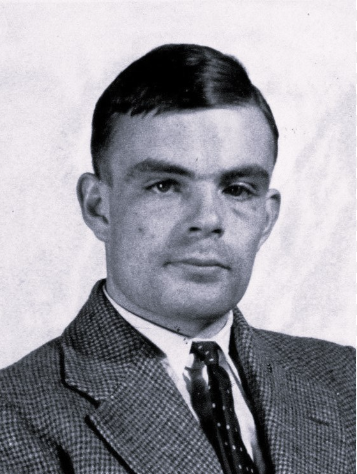
\includegraphics[width=0.5\linewidth]{figuras/alan_turing.png}
        \caption{Alan Turing}
        \label{fig:image2}
    \end{subfigure}
    \caption{Jhon Maccarthy e Alan Turing}
    \label{fig:figures}
\end{figure}

Foi na década de 1970 que o uso da IA começou a ser mais difundido. Uma das primeiras abordagens foram os Sistemas Especialistas (SE). Eles dependiam muito dos especialistas do domínio para transformar o conhecimento tácito (baseado em sua experiência) em explicito (formalizado, documentado), que era então codificado na forma de regras em lógica formal. O processo de aquisição desse conhecimento acabou sendo um grande obstáculo na adoção em massa dessa abordagem. Veja um exemplo de software que implementa um motor de inferência baseado na teoria dos sistemas especialistas na Figura~\ref{fig:expert}

\begin{figure}
	\centering
	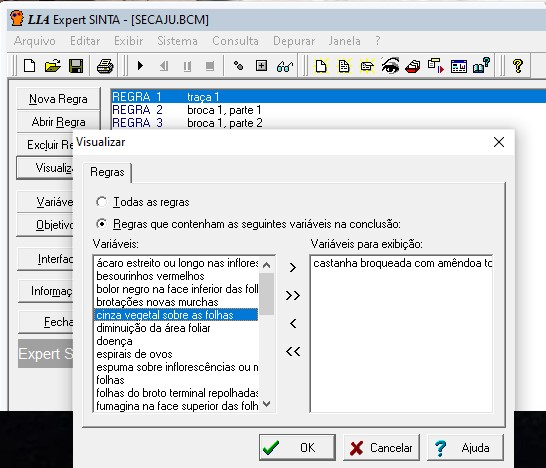
\includegraphics[width=0.7\linewidth]{figuras/expert}
	\caption{ExpertSinta. Uma interface de um Sistema Especialista}
	\label{fig:expert}
\end{figure}

Nestas últimas décadas houve um crescimento exponencial das tecnologias que  estão ao redor da IA, tais como, o aumento da capacidade de processamento e armazenamento dos computadores, a geração de grandes volumes de dados, avanços científicos e tecnológicos, chips supercondutores, eficiência energética. Isso permitiu avanços significativos que até então esbarravam em limitações.

\section{Aprendizado de Máquina}

O Aprendizado de Máquina (AM) é uma subárea da IA (Figura~\ref{fig:iaam}). que foi motivada pelo desenvolvimento de softwares mais independentes da intervenção humana para extração do conhecimento, o que era uma dificuldade nos Sistemas Especialistas. Geralmente aplicações de AM utilizam \textbf{heurísticas} (regra do dedão) que buscam por modelos capazes de representar o conhecimento existente nos dados.

%% TODO: Definir melhor heurística

\begin{figure}
	\centering
	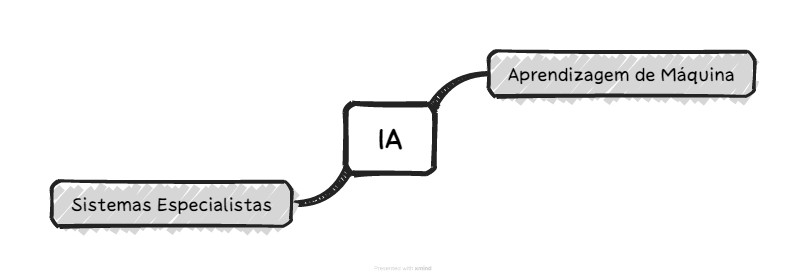
\includegraphics[width=0.9\linewidth]{figuras/ia.png}
	\caption{AM é uma parte da IA}
	\label{fig:iaam}
\end{figure}

Na Figura~\ref{fig:exemplosam}, é possível identificar alguns usos de AM integrado em diversas atividades cotidianas. São elas, (a) Um smartphone com um assistente de voz fornecendo atualizações meteorológicas. (b) Um sistema de casa inteligente ajustando o termostato com base nas preferências do usuário. (c) Um carro autônomo dirigindo em uma rua movimentada da cidade. (d) Uma plataforma de compras online recomendando produtos a um usuário com base em suas compras anteriores. Essa figura foi criada inclusive com inteligência artificial.

\begin{figure}
	\centering
	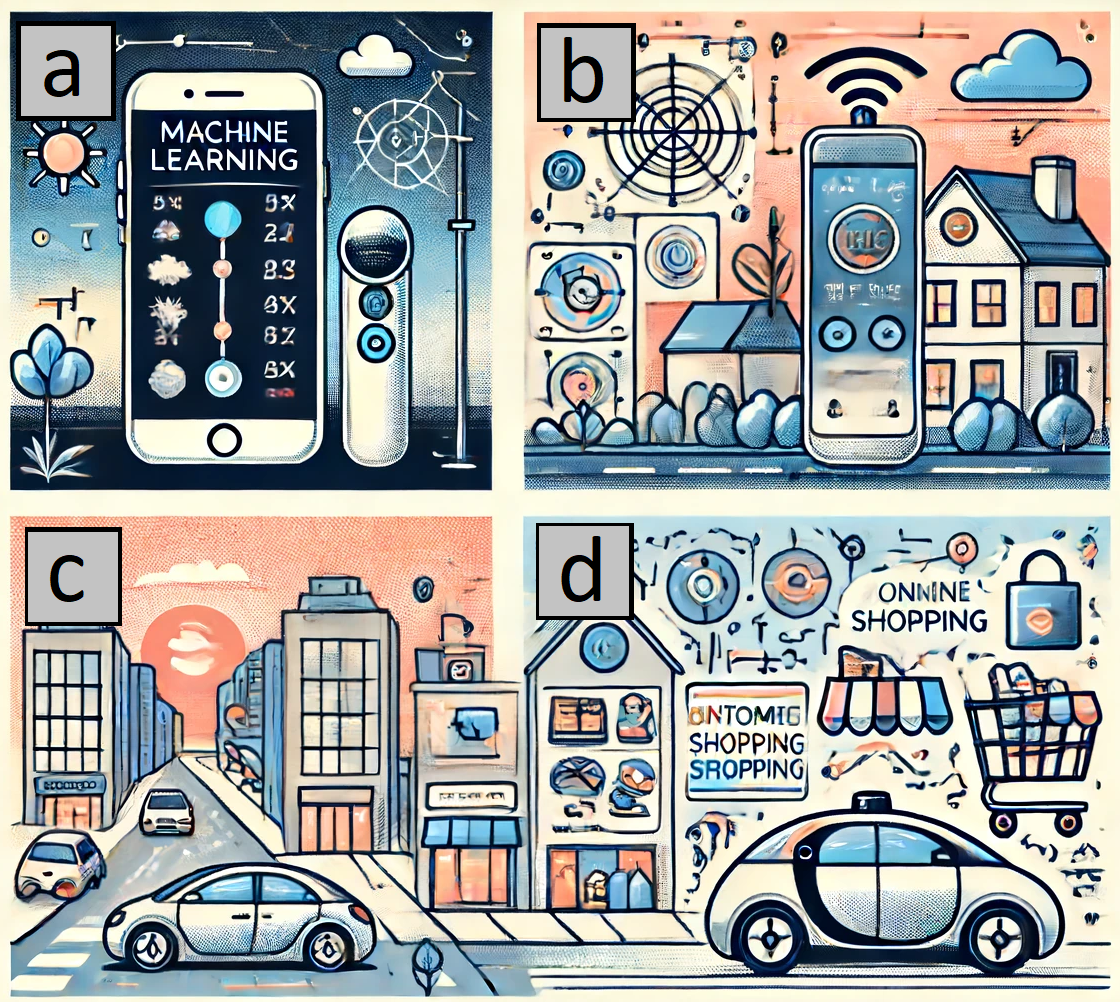
\includegraphics[width=0.7\linewidth]{figuras/exemplos_am}
	\caption{Exemplos AM}
	\label{fig:exemplosam}
\end{figure}

\subsection{Classificação}

As tarefas de aprendizado de máquina podem ser divididas entre tarefas preditivas, que visam inferir o atributo alvo de uma nova entrada a partir da exposição prévia aos dados rotulados durante o treinamento do modelo, e descritivas, que buscam extrair padrões dos atributos preditivos. Por conseguinte, uma vez que pertencem a este paradigma, as tarefas de aprendizado descritivas não possuem atributos alvo. Noutras palavras, tarefas preditivas analisarão os atributos preditivos, comparando-os com os atributos alvo (rótulos), ao passo que tarefas descritivas utilizaram os atributos preditivos entre si para buscar por padrões e correlações.

\begin{figure}
	\centering
	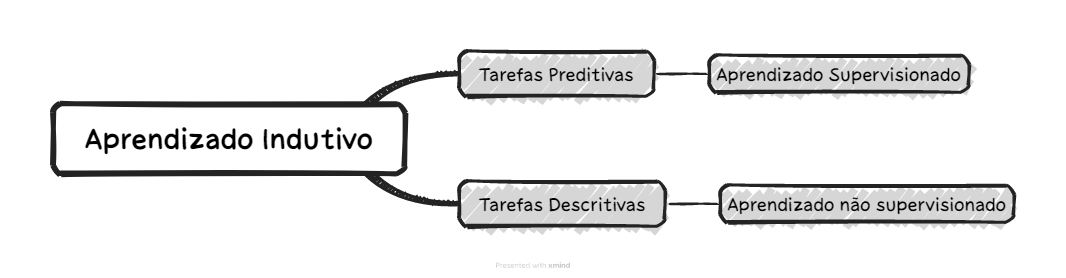
\includegraphics[width=1\linewidth]{figuras/indutivo.png}
	\caption{Classificação AM}
	\label{fig:indutivo}
\end{figure}

Ambas as tarefas podem ser categorizadas sob o conceito de aprendizado indutivo, que é a capacidade de generalizar a partir de exemplos específicos, isto é, do conjunto de dados de treinamento. Em se tratando de tarefas preditivas, os algoritmos poderão implementar tarefas de classificação, nas quais o atributo alvo (rótulo) é discreto (enumerável ou finito), ou de regressão, em que o atributo alvo (rótulo) é contínuo (não enumerável ou infinito). Já as descritivas distinguem-se entre agrupamento, que busca por similaridades, associação, que busca por padrões frequentes, e sumarização, que resulta em um resumo do conjunto de dados.

% TODO: sinonimo supervisionado e não supervisionado

\subsection{Exemplo de AM com Python}

A seguir um exemplo de modelo preditivo em Python. O modelo utiliza o algoritmo SVM e o conjunto de dados iris, que é um conjunto de dados conhecido e bastante utilizado como em demonstrações em outros livros e sites.

\begin{lstlisting}[language=Python, caption={Exemplo de código que usa AM}]
	from sklearn import svm
	from sklearn.datasets import iris
	iris = load_iris()
	X = iris.data
	y = iris.target
	model = svm.SVC()
	model.fit(X, y)
	model.predict([[2., 2., 2., 2.]])
\end{lstlisting}

%\chapter{Modelo Preditivo}

%\section{Intuição de um modelo preditivo}

%\section{Exemplo de Código}

%Aqui está um exemplo de código em Python:

%\begin{lstlisting}[language=Python, caption={Exemplo de Código Python}]
%	def hello_world():
%		print("Hello, world!")
%
%	hello_world()
%\end{lstlisting}

\chapter{Estatística Básica}

Um conjunto de dados geralmente é uma estrutura tabular com linhas e colunas, o nome da coluna é o identificador do dado (também chamado de variável) disposto naquela coluna. Cada linha da coluna é chamada de observação (ou registro), e representa uma instância daquele elemento. Por exemplo, uma tabela com dados do cliente é apresentado na Tabela~\ref{tbl:cliente}, a primeira linha (em negrito) é o nome da coluna, são elas: nome, endereço e telefone; cada linha abaixo do nome da coluna representa um cliente. Portanto a linha 1, teria o nome das 3 colunas; já a linha 2, teria um determinado cliente, e a linha 3, outro cliente.

\begin{table}
	\centering
	\caption{Tabela cliente.}
	\begin{tabular}{|l|l|c|}
	\hline
	\textbf{Nome} & \textbf{Endereço} & \textbf{Telefone} \\
	\hline
	Giseldo Neo & Rua das alamedas, n 27, Corumbá MS & 222 66666 \\
	\hline
	Alex Neo & Avenida Fernandes 325, Macieó, AL& 333 6589 \\
	\hline
	\end{tabular}
	\label{tbl:cliente}
\end{table}

Em resumo, a Tabela~\ref{tbl:cliente} apresenta 2 observações (ou registros) de clientes. A primeira coluna é uma descrição das informações que existirão naquela coluna, por exemplo ``nome'' significa que provavelmente todos os dados dessa coluna são referentes ao nome de determinado cliente, já cada linha abaixo da primeira linha são os dados de um cliente em específico.

Quando vamos realizar um resumo estatístico (tal como média, mediana ou moda), ou algum gráfico, ou alguma inferência estatística, ou rodar um modelo preditivo, temos que conhecer o tipo teórico, daquele dado (ou variável, ou coluna) para podermos selecionar qual a técnica mais adequada que devemos aplicar. Por exemplo, em nenhuma das colunas da tabela cliente devemos calcular a média. Qual é a média, do nome? ou a média do endereço, ou a média do telefone? Não faz sentido.

Utilizando uma classificação para esse tipo de variável, podemos definir qual é o tipo possível de operação. Portanto, vamos acrescentar mais uma informação (teórica) a coluna da tabela para que possamos claramente definir o que deve, ou pode ser feito com ela, chamamos essa informação de tipo de dado, ou tipo de variável, que é o termo mais usado.

Conhecendo estes tipo e sua aplicação correta não cometeremos o erro de por exemplo, calcular a média de uma variável do tipo qualitativa ordinal. Além disso, é interessante reportar nos estudos científicos (artigos) uma tabela com o tipo das variáveis utilizado, pois isso facilita muito o entendimento do conjunto dos dados para o leitor interessado, caso o artigo tenha utilizado um conjunto de dados.

\section{Variável}

Uma variável, em conceitos estatísticos, é uma característica do que foi observado naquele universo (amostra ou população), que foi medida,  contada, ou categorizada \cite{favero2017manual}. No nosso exemplo do cliente (Tabela~\ref{tbl:cliente}) as variáveis são: nome, endereço e telefone. Elas foram registradas na tabela após um desses processos de mensuração, contagem ou categorização. Por exemplo, medimos a altura de uma pessoa e registramos isso em uma tabela, a altura é então chamada genericamente de variável.

É útil definir de qual tipo é determinada variável, pois, existem técnicas adequadas para cada tipo. Para realizar uma análise estatística descritiva, elaborar um gráfico para um artigo científico, ou aplicar uma técnica de pré-processamento em um modelo preditivo é necessário entender de qual tipo é cada variável, pois existem determinadas técnicas para determinados fins. Por isso, vamos entender estas classificações teóricas.

Neste contexto, uma variável pode ser \textbf{quantitativa} ou \textbf{qualitativa} (Figura~\ref{fig:tipodado}). Além disso, uma variável quantitativa também é chamada de métrica, e a variável qualitativa de não métrica ou categórica \cite{favero2017manual}.

\begin{figure}
	\centering
	\caption{Classificação da variável}
	\begin{tikzpicture}
		\draw
		node[draw] at (0,2) (tipo) {Variável}
		node[draw] at (-3,0) (quan) {Quantitativa}
		node[draw] at (3,0) (quali) {Qualitativa};
		\draw[->] (tipo) -- (quan);
		\draw[->] (tipo) -- (quali);
	\end{tikzpicture}
	\label{fig:tipodado}
\end{figure}

A variável quantitativa é expressa geralmente como um número. Porém, existem casos em que números também expressam variáveis qualitativas, logo cada caso deve ser analisado individualmente. Já a variável do tipo qualitativa está relacionado ao pertencimento do valor mensurado a um universo. Um exemplo de variável qualitativa é o estado civil do cliente, que pode ser solteiro ou casado. Para continuarmos, vamos atualizar nossa tabela de cliente com duas novas variáveis, estado civil e altura, assim teremos variáveis dos tipos qualitativa e quantitativas  na mesma tabela, o que é bem comum (Tabela~\ref{tbl:cliente_v2}).

\begin{table}
	\centering
	\caption{Tabela cliente atualizada com novas colunas e novos registros.}
	\begin{tabular}{|l|l|c|c|c|}
	\hline
	\textbf{Nome} & \textbf{Endereço} & \textbf{Telefone} & \textbf{Estado civil} & \textbf{Altura} \\
	\hline
	Giseldo Neo & Rua das Alam[..] & 222 66666 & casado & 1,80\\
	\hline
	Alex Barros & Avenida Ferna[..]& 333 6589 & solteiro & 1,70 \\
	\hline
	Pedro Alves & Alameda dos Anj[..]& 888 5879 & casado & 1,50 \\
	\hline
	Miguel Peixoto & BR 259, trecho[..]&  & solteiro & 1,79 \\
	\hline
	\end{tabular}
	\label{tbl:cliente_v2}
\end{table}

Para exemplificar, tipificaremos (ou classificaremos) as variáveis (ou  características) que foram medidas, contadas (com determinado grau de precisão) ou categorizadas dos clientes em uma outra tabela para registrar estes dados sobre as variáveis (se quantitativo ou qualitativo). Veja na Tabela~\ref{tbl:clienteclassificacao} o resultado dessa tipificação, para cada variável informamos se a variável é qualitativa ou quantitativa na segunda coluna, já na primeira coluna temos o nome da variável.

\begin{table}
	\centering
	\caption{Tipo das variáveis da tabela cliente.}
	\begin{tabular}{|c|c|}
		\hline
		\textbf{Nome da variável} &\textbf{Tipo da variável} \\
		\hline
		Nome & qualitativa \\
		\hline
		Endereço & qualitativa \\
		\hline
		Telefone & qualitativa \\
		\hline
		Estado Civil & qualitativa \\
		\hline
		Altura & quantitativa \\
		\hline
	\end{tabular}
	\label{tbl:clienteclassificacao}
\end{table}

No entanto, ainda temos uma outra classificação das variáveis, relacionada as \textbf{escalas}. As escalas são 3: \textbf{mensuração}, \textbf{precisão} (da contagem) e \textbf{categorização}. As opções da escala mensuração são: \textbf{intervalar} e \textbf{razão} para as variáveis quantitativas e \textbf{nominal} e \textbf{ordinal} para as variáveis qualitativas. Veja na Figura~\ref{fig:mensuracao}, o tipo das variáveis e as escalas de mensuração de cada tipo. Além das escalas de mensuração, temos as escalas de precisão e as escalas de categorização. A escala de precisão é utilizada somente nas variáveis quantitativas com as opções \textbf{discreta} ou \textbf{contínua}. Já a escala de categorização é utilizada somente em variáveis qualitativas, suas opções são \textbf{binária} ou \textbf{policotômica}.

\begin{figure}
	\caption{Escala da variável}
	\centering
	\begin{tikzpicture}
		\draw
		node[draw] at (0,2) (esc) {Escala}
		node[draw, red] at (-6,0) (men) {Mensuração}
		node[draw, blue] at (0,0) (pre) {Precisão (da contagem)}
		node[draw, green] at (4,0) (cat) {Categorização}
		node[draw, red] at (-9,-2) (int) {Intervalar}
		node[draw, red] at (-7,-2) (raz) {Razão}
		node[draw, red] at (-5,-2) (nom) {Nominal}
		node[draw, red] at (-3,-2) (ord) {Ordinal}
		node[draw, blue] at (-1,-2) (dis) {Discreta}
		node[draw, blue] at (1,-2) (con) {Contínua}
		node[draw, green] at (3,-2) (bin) {Binária}
		node[draw, green] at (5.3,-2) (pol) {Policotômica}
		[->] (esc) -- (men)
		[->] (esc) -- (pre)
		[->] (esc) -- (cat)
		[->] (esc) -- (men)
		[->] (men) -- (int)
		[->] (men) -- (raz)
		[->] (men) -- (nom)
		[->] (men) -- (ord)
		[->] (pre) -- (dis)
		[->] (pre) -- (con)
		[->] (cat) -- (bin)
		[->] (cat) -- (pol);
\end{tikzpicture}
	\label{fig:mensuracao}
\end{figure}



\begin{figure}
	\caption{Escala de \textcolor{red}{mensuração}, \textcolor{blue}{precisão} e \textcolor{green}{categorização} das variáveis quantitativa e qualitativa}
	\centering
	\begin{tikzpicture}
		\draw
		node[draw] at (0,2) (tipo) {Variável}
		node[draw] at (-3,0) (quan) {Quantitativa}
		node[draw] at (5,0) (qual) {Qualitativa}
		node[draw, red] at (-6,-2) (int) {Intervalar}
		node[draw, red] at (-4,-2) (raz) {Razão}
		node[draw, blue] at (-2.1,-2) (dis) {Discreta}
		node[draw, blue] at (0,-2) (con) {Continua}
		node[draw, red] at (4,-2) (nom) {Nominal}
		node[draw, red] at (2,-2) (ord) {Ordinal}
		node[draw, green] at (5.8,-2) (bin) {Binaria}
		node[draw, green] at (8,-2) (pol) {Policotômica}
		[->] (tipo) -- (quan)
		[->] (tipo) -- (qual)
		[->] (quan) -- (dis)
		[->] (quan) -- (con)
		[->] (qual) -- (bin)
		[->] (qual) -- (pol)
		[->] (quan) -- (raz)
		[->] (quan) -- (int)
		[->] (qual) -- (ord)
		[->] (qual) -- (nom);
	\end{tikzpicture}
	\label{fig:mensuracao}
\end{figure}

Portanto se a variável for quantitativa ela somente poderá ser ou intervalar ou razão, além disso, discreta ou continua. Se ela for qualitativa, ela poderá ser ordinal ou nominal, também  binaria ou policotônica. Em outras palavras ela só terá duas dessas classificações de escala, se estivessemos lidando com cores, bastaria escolher uma opção da cor vermelha e uma da cor azul, se for quantitativa, e uma da cor vermelha e outra da cor verde se qualitativa. A Tabela~\ref{tbl:clienteclassificacaoescala} está atualizada com essa classificação das escalas.

\begin{table}
	\centering
	\caption{Classificação das variáveis, agora com as escalas.}
	\begin{tabular}{|l|l|}
		\hline
		\textbf{Nome da variável} &\textbf{Classificação} \\
		\hline
		Nome & qualitativa, nominal e policotômica  \\
		\hline
		Endereço & qualitativa, nominal e policotômica  \\
		\hline
		Telefone & qualitativa, nominal e policotômica \\
		\hline
		Estado Civil & qualitativa, nominal e binaria \\
		\hline
		Altura & quantitativa, intervalar e continua \\
		\hline
	\end{tabular}
	\label{tbl:clienteclassificacaoescala}
\end{table}

\subsection{Quantitativa}

Já sabemos que uma variável quantitativa é expressa geralmente (mas nem sempre) como um número, e pode ser quanto a sua escala de mensuração, intervalar ou razão. Além disso, essa variável ainda pode ser classificada em relação a sua escala de precisão, contínuo ou discreto.

Sabendo que a variável é quantitativa podemos utilizar as medidas estatísticas de posição ou localização, tais como, média, mediana, moda, quartis, decis e percentis. Também podemos utilizar as medidas de dispersão, tais como, amplitude, desvio padrão, erro-padrão e coeficiente de variação. Além disso, para uma representação visual dos gráficos podemos utilizar os gráficos do tipo linha, dispersão, histograma, ramo-e-folhas e boxplot, por fim as medidas de forma como assimetria e curtose também podem ser utilizadas\cite{favero2017manual}.

\subsubsection{Escala de precisão: Quantitativa contínua}

A  variável quantitativa, com escala de precisão contínua, é quando ela possui um intervalo de domínio dos números reais. Lembrando que o conjunto de número reais engloba os números inteiros. Geralmente essa variável é o resultado de uma medida, por exemplo, a altura dos estudantes é um dado do tipo quantitativo contínuo.

Vamos criar em Python uma tabela (chamado de DataFrame) que tem uma única coluna (variável) do tipo quantitativa continua. Porém, as linguagens (Python, R) ou as ferramentas estatísticas visuais (tais como: SPSS, JASP ou Jamovi), não são obrigadas a ter um equivalente dessa tipologia teórica, isso depende do contexto do dado, da interpretação humana do que aquela variável representa. No código a seguir criamos uma tabela com uma única coluna. Classificamos então ela em relação a escala de precisão (da contagem) como continua. Em programação o termo variável é utilizado para um fim diferente, porém nesse capítulo, quando falamos de variável estamos nos referindo a coluna da tabela.

\begin{lstlisting}[language=Python, caption={Código que cria e exibe uma tabela em python com uma variável quantitativa continua.}]
>>> import pandas as pd
>>> dados = [1.80, 1.70, 1.50, 1.79]
>>> df = pd.DataFrame(data=dados, columns=['altura'])
>>> df
   altura
0    1.80
1    1.70
2    1.50
3    1.79
>>>
\end{lstlisting}

\begin{comment}

\subsubsection{Escala de precisão: Quantitativa discreto}

O dado numérico discreto geralmente é resultado de uma contagem - um número inteiro. Por exemplo, a idade é uma contagem de anos do estudante, logo é um dado do tipo \textbf{numérico discreto}.

Por exemplo, a idade de um estudante é um dado do tipo \textbf{numérico discreto}.

Cada linguagem de programação tem tipos de dados específicos para suas variáveis, que estão relacionados as vezes com essa classificação teórica (numérico contínuo ou numerico discreto). Por exemplo no python temos o tipo da variável \textit{int} (inteiro), que é equivalente ao numerico discreto, já o tipo \textit{float} (flutuante) é equivalente ao numérico contínuo.

Aqui está um exemplo de código em Python:

\begin{lstlisting}[language=Python, caption={Exemplo de declaração de variável do tipo inteiro, equivalente ao tipo de dado numérico contínuo.}]
	>>> idade = 25
	>>> type(idade)
	<class 'int'>
\end{lstlisting}

\subsection{Dado qualitativo}

Um dado é do tipo categórico quando ele faz parte de um conjunto, de uma classe ou de uma categoria.

O dado categórico pode ser binário ou ordinal, ou nenhuma das duas subcategorias.

Um exemplo de dado categórico, é uma lista com as cores preferidas dos estudantes, ou o estado civil de uma pessoa.

O dado do tipo categórico binário é um tipo especial quando ele somente pode assumir dois valores no universo de valores possíveis. Por exemplo 0 ou 1, existente ou ausente, true ou false, sim e não.

O dado do tipo categórico ordinal também é um tipo especial, é quando ele faz parte de um conjunto com determinada ordem, por exemplo, imagine a classificação de altura de estudantes somente com os valores alto, médio e baixo. Nesse exemplo existe uma ordem, o aluno com altura classificado como baixo tem uma altura menor do que o aluno com altura média.}
\end{comment}

\bibliographystyle{apalike}
\bibliography{ref}

\end{document}